\newpage
\section*{Appendix B}
\label{appendix_b}
%Isaac Meza
\setcounter{table}{0}
\renewcommand{\thetable}{B.\arabic{table}} 
\setcounter{figure}{0}
\renewcommand{\thefigure}{B.\arabic{figure}} 

\title{\Large{\textbf{The Effect of Agency on Settlement Rates}}}

We aim to write down a simple model that aims to illuminate why agency issues plausibly the underlying cause of the patterns in treatment we find on Tables \ref{Treatment_effects} and \ref{te_bylawyer}. The treatment is effective only when plaintiffs are present to receive it directly. Moreover, this pattern is driven by cases where the plaintiff is represented by a private lawyer. These basic facts could be explained by several models, and we do not claim that the simple and highly stylized framework we write down here is the only way to rationalize them.

Private lawyers almost always receive a share of whatever the plaintiff collects. We should expect the contingency payment contract to align incentives with regard to effort at least partially. We focus instead on differences in incentives over the decision to settle or proceed with the case.  The parties differ in their ability to diversify risks and are also likely to have different discount rates. Our framework focuses on these differences, and shows why they may lead to differences in preferences over taking a certain payoff now (i.e., a settlement) or an uncertain payoff later (i.e., a court judgment). 

 We start with three utility functions, $\left(U_w(x), U_l(x), U_f(x)\right)$, defined over the amount awarded to plaintiffs for the plaintiff ($w$), the plaintiff's lawyer ($l$), and the firms($f$)\footnote{We will assume that $U(0)=0$, $U^{\prime}(x)>0$ and $U^{\prime\prime}(x)\leq 0$, so that $U$ is risk averse or risk neutral. We can think of the 30 percent of any recovery that the plaintiffs' lawyers typically receive as being already reflected in their utility function.}, and subjective distributions $g_k(x)$ for $k=\{w,l,f\}$ for the amount that party $k$ recovers (pays) in a trial. We define the \emph{settlement range} between the plaintiff and defendant as $I_{w,f}:=\left\{x\;\;|\;\;\mathbb{E}_wU_w\leq x\leq\mathbb{E}_fU_f\right\}$, where expectations are taken with respect to $g_k(x)$ and the utility functions incorporate attitudes toward risk over uncertain outcomes. If the utility over outcomes differs for plaintiffs and their lawyers, then we can also define a similar settlement range between firms and plaintiff's lawyers as $I_{l,f}:=\left\{x\;\;|\;\;\mathbb{E}_lU_l\leq x\leq\mathbb{E}_fU_f\right\}$. 

We show three claims that follow from this simple framework.

\begin{claim}
\label{claim1}
Suppose $g_w(x)=g_l(x)=g_f(x):=g(x)$  and 
\[A_{U_w}(x)\geq A_{U_l}(x)\geq A_{U_f}(x)\quad ;\;\forall\;x\in \operatorname{supp} g \]
where $A_{U}(x)-\frac{U^{\prime\prime}(x)}{U^{\prime}(x)}$ is the Arrow-Pratt measure of risk aversion. Suppose further that $U_w^{\prime}(x)\leq U_l^{\prime}(x)\leq U_f^{\prime}(x)$ in a neighbourhood of $0$. Then $\emptyset\neq I_{l,f}\subseteq I_{w,f}$. That is, the worker is more willing to settle than her lawyer.
\end{claim}

\textit{Proof of claim (\ref{claim1}):}
It will suffice to prove that $\mathbb{E}_wU_w\leq \mathbb{E}_lU_l\leq \mathbb{E}_fU_f$. 

Now, 
\begin{align*}
A_{U_w}(x)\geq A_{U_l}(x)\; \Longleftrightarrow & \; \frac{U_w^{\prime\prime}(x)}{U_w^{\prime}(x)}\leq \frac{U_l^{\prime\prime}(x)}{U_l^{\prime}(x)} \\
\Longleftrightarrow \; & \frac{d}{dx}\ln(U_w^{\prime}(x))\leq \frac{d}{dx}\ln(U_l^{\prime}(x))\\
\;\Longleftrightarrow & \int_0^{y}\frac{d}{dx}\ln(U_w^{\prime}(x))dx\leq \int_0^{y}\frac{d}{dx}\ln(U_l^{\prime}(x))dx \;\;\forall\; y\in\;\operatorname{supp}g\\
\Longleftrightarrow \; & \ln(\frac{U_w^{\prime}(y)}{U_w^{\prime}(0)})\leq \ln(\frac{U_l^{\prime}(y)}{U_l^{\prime}(0)})\;\;\forall\; y\in\;\operatorname{supp}g\\
\; \Longleftrightarrow & \frac{U_w^{\prime}(y)}{U_w^{\prime}(0)}\leq \frac{U_l^{\prime}(y)}{U_l^{\prime}(0)}\;\;\forall\; y\in\;\operatorname{supp}g \\
\Longrightarrow \; & U_w^{\prime}(y)\leq U_l^{\prime}(y)\;\;\forall\; y\in\;\operatorname{supp}g
\end{align*}

As $U(0)=V(0)$ the last inequality tells us that
\[U_w(x)\leq U_l(x)\;\;\forall\; x\in\;\operatorname{supp}g\]
 which together with the fact that all parties follow the same subjective distribution leads to 
 \[\mathbb{E}_wU_w\leq \mathbb{E}_lU_l\]
 The other inequality is proved analogously.


Claim 1 says that even with the same subjective $g(x)$ for all parties, if plaintiffs are more risk averse than defendants\footnote{Since the workers typically have much lower incomes and have recently lost a job, and since both the plaintiff's lawyers and the firms typically manage several cases simultaneously, we believe this is a reasonable assumption. With a slightly more complex model, we can get the same result even with the same utility function for the lawyer and the worker, if lawyers are able to diversify across multiple cases. Since, on average, lawyers surveyed in phase 1 reported having more than 100 open cases, we think it is safe to say that lawyers are far more diversified than workers.} then the settlement range between the worker and firm is non empty. Moreover, if the worker is more risk averse than her lawyer, then the settlement range between the firm and the plaintiff's lawyer is a subset of the settlement range between the firm and the plaintiff. Therefore, the worker will be willing to accept some settlement offers that her lawyer will want to reject. The difference in the circumstances governing risk creates a potential conflict of interest between the plaintiff and her own lawyer. 

\begin{claim}
\label{claim2}
Assume additionally that $g^o_w \succeq_{FOSD} g_w$. Then $I_{w^o,f} \subseteq I_{w,f}$. That is, overconfidence shrinks the settlement range.
\end{claim}

\textit{Proof of claim (\ref{claim2}):}
As $g^o_w$ first-order stochastically dominates $g_w$ then 
\[\mathbb{E}_{g^o_w}U\geq \mathbb{E}_{g_w}U\]
for all weakly increasing $U$. From this the claim follows directly.


Claim 2 relaxes the assumption of the same expectations over outcomes to allow for overconfidence. We show that if the worker is overconfident (i.e. $g_w^o$ first-order stochastically  dominates $g_w$) then the settlement range shrinks. Indeed, if the parties are sufficiently optimistic, the settlement range will be empty. Our surveys in phase 3 indicate that workers are wildly optimistic before filing a case. Because most workers are suing for the first time, while their lawyers have typically handled a large number of cases, the lawyers have the ability to guide workers toward realistic expectations or maintain their initial overconfidence. The misalignment between the worker and her lawyer generated by Claim 1 gives an incentive for the lawyer to inflate the expectations of the worker. 

\begin{claim}
\label{claim3}
Let the worker have a prior distribution $g_w$, and let the calculator be a signal with distribution $S$. Suppose further that the signal satisfies  $g_w \succeq_{FOSD} S$ and that the agent is Bayesian. If we denote the posterior by $\hat{g}_w$, then $I_{w,f} \subseteq I_{\hat{w},f}$. That is, after updating the settlement range increases.
\end{claim}
%\footnote{We say that the agent is Bayesian if he follow a \emph{Bayesian rule} according to definition in \textit{Shmaya \& Yariv. Foundations for Bayesian Updating.}}

\textit{Proof of claim (\ref{claim3}):}
We will prove that  $g_w \succeq_{FOSD} \hat{g}_w \succeq_{FOSD} S$, combining this fact with Claim \ref{claim2} will yield the desired result.

As the agent is Bayesian, then by Theorem 1 in \textit{Foundations for Bayesian Updating} we can write $\hat{g}_w=\alpha g_w+(1-\alpha)S$ for some $\alpha\in [0,1]$. Then,

\[\mathbb{E}_{\hat{g}_w}U=(1-\alpha)\mathbb{E}_{g_w}U+\alpha \mathbb{E}_{S}U\leq(1-\alpha)\mathbb{E}_{S}U+\alpha \mathbb{E}_{S}U= \mathbb{E}_{S}U\]
for all weakly increasing $U$. As $S$ is dominated by $g_w$, this yields the desired inequality.


Claim 3 introduces the calculator as a signal received by Bayesian updaters, and shows that when initially overconfident workers get the calculator, their settlement range increases to $\hat{I}_{w,f}$, leading to more settlements.

The effect of the three claims can be illustrated in the following figure, which shows the effect of overconfidence and differences in the ability to diversify risk on the settlement range over which parties might bargain a resolution to the case.  

\begin{figure}[H]
   \caption{Illustration of claims}
   \label{figure}
\begin{center}
 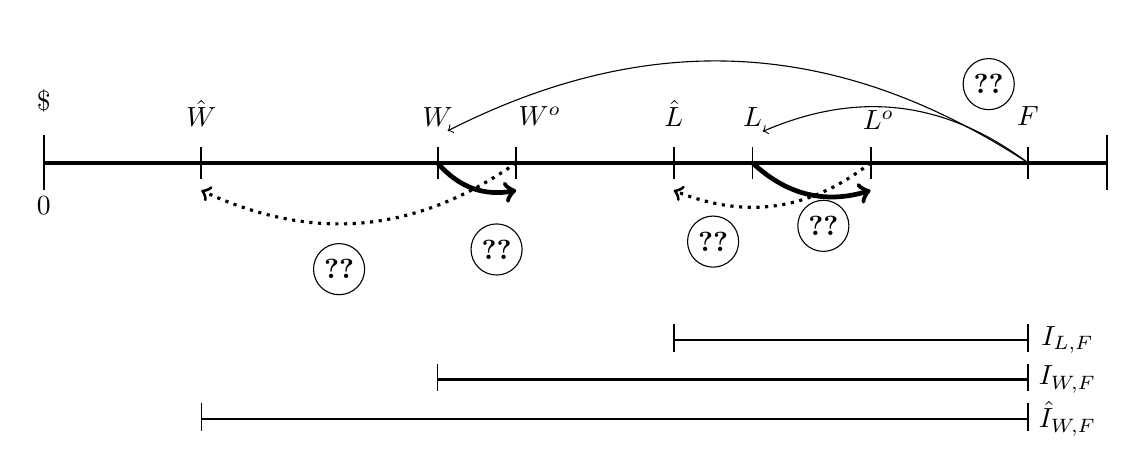
\begin{tikzpicture}
    \draw[line width=0.5mm] (0,0) -- (13.5,0) node [below] {};
    \foreach \x in {0,13.5}
    \draw[line width=0.3mm] (\x, 0.35) -- node[pos=-0.25] (point\x) {} (\x, -0.35);
    
    \foreach \x in {2, 5, 6, 8, 9, 10.5, 12.5}
    \draw[line width=0.25mm] (\x, 0.2) -- node[pos=-0.35] (point\x) {} (\x, -0.2);
    % node's content --- access them as point1...point5
    \path (point0) node [above] {$\$$};
    \path (0,-0.3) node [below] {$0$};
    \path (point2) node [above] {$\hat{W}$};
    \path (point5) node [above] {$W$};
    \path (6.3,0.35) node [above] {$W^o$};
    \path (point8) node [above] {$\hat{L}$};
    \path (point9) node [above] {$L$};
    \path (10.6,0.3) node [above] {$L^o$};
    \path (12.5,0.35) node [above] {$F$};
    
    \path (12.5,0) edge[black, bend right, ->] (point9);
    \path (12.5,0) edge[black, bend right, ->] (point5);
    \draw (12,1) node[circle,draw, inner sep=2pt](c1) {$\ref{claim1}$};
    
    \path (5,0) edge[black, line width=0.6mm, bend right, below, ->] (6,-0.35);
    \draw (5.75,-1.1) node[circle,draw, inner sep=2pt](c2) {$\ref{claim2}$};
    
    \path (9,0) edge[black, line width=0.6mm, bend right, below, ->] (10.5,-0.35);
    \draw (9.9,-0.8) node[circle,draw, inner sep=2pt](c2) {$\ref{claim2}$}; 
    
    \path (6,0) edge[black, line width=0.4mm, dotted, bend left, below, ->] (2,-0.35);
    \path (3.75,-1.35) node[circle,draw, inner sep=2pt]  {$\ref{claim3}$};

    
    \path (10.5,0) edge[black, line width=0.4mm, dotted, bend left, below, ->] (8,-0.35);
    \draw (8.5,-1.0) node[circle,draw, inner sep=2pt] {$\ref{claim3}$};  

    
    \draw[line width=0.3mm] (8,-2.25) -- (12.5,-2.25) node [below] {};
    \foreach \x in {8,12.5}
    \draw[line width=0.2mm] (\x, -2.05) -- node[pos=-0.25] {} (\x, -2.4);
    \path (13,-2.25) node  {$I_{L,F}$};
    
    \draw[line width=0.3mm] (5,-2.75) -- (12.5,-2.75) node [below] {};
    \foreach \x in {5,12.5}
    \draw[line width=0.2mm] (\x, -2.55) -- node[pos=-0.25] {} (\x, -2.9);
    \path (13,-2.75) node  {$I_{W,F}$}; 
    
    
    \draw[line width=0.3mm] (2,-3.25) -- (12.5,-3.25) node [below] {};
    \foreach \x in {2,12.5}
    \draw[line width=0.2mm] (\x, -3.05) -- node[pos=-0.25] {} (\x, -3.4);
    \path (13,-3.25) node  {$\hat{I}_{W,F}$}; 
    
  \end{tikzpicture}
 \end{center}

\scriptsize
    \textit{Notes:} 
    To simplify the notation we will simply write the subindex $i\in \lbrace W, L , F\rbrace$ to denote $\mathbb{E}_iU_i$. The arrows describe the conclusion on each of the claims: Initially with the same subjective probability but with different degrees of risk aversion, the expected utility of the different parties differ. This is Claim \ref{claim1}. Claim \ref{claim2} tells us that for overconfident individuals (here denoted by $W^o$), their expected utility increases. Finally, Claim \ref{claim3} is about the updating process for lawyers and workers, assuming that the calculator reduces the overconfidence. The conclusion is that after updating, the settlement range increases.  The last intervals denote the \emph{settlement range}, the first one for the lawyer and the last two before and after updating, when the employee is present. 
\end{figure} 








